\lecture{10}{20 Nov. 14:20}{}

考慮 Ford-Fulkerson algorithm 的複雜度分析,如果所有容量都是整數,則每次增廣至少增加 1 單位的流量,而 $m$ 條管線的容量總和是 $C = \sum_{e \in E} c(e)$,因此最多增廣 $C$ 次,每次找增廣路徑花費$O(m)$的時間,總複雜度是 \[
    T(m, C) = O(C) \cdot O(m) = O(mC)
\]
但,這個算是「多項式時間」(polynomial time)演算法嗎?還是是「指數時間」(exponential time)演算法?
\begin{remark}
    Complexity is according to the input size of an instance.
\end{remark}

\begin{eg}
    For an $n \times n$ matrix multiplication problem, the input size is $N = \Theta(n^2)$ (set all the number is of size $O(1)$).
\end{eg}

The complexity is 
\begin{itemize}
    \item Linear-time if $T(N) = O(N) = O(n^2)$.
    \item Quadratic-time if $T(N) = O(N^2) = O(n^4)$.
    \item Polynomial-time if $T(N) = O(N)^{O(1)} = O(n)^{O(1)}$.
    \item Exponential-time if $T(N) = O(1)^N = O(1)^{n^2}$ or more.
\end{itemize}

\begin{definition}[Complexity of Linear/Quadratic/Polynomial-time Algorithms]
For any instance $I$,define its input size as a non-negative integer function
\[
    N = \mathrm{size}(I),
\]
其中 $N$ 表示描述輸入實例所需的位元數或其他適當的度量方式。
令 $T(N)$ 為某演算法在輸入大小為 $N$ 時的最壞情況執行時間。我們對時間複雜度作如下分類:
\begin{itemize}
    \item Linear-time algorithm:若 $T(N) = O(N)$。
    \item Quadratic-time algorithm:若 $T(N) = O(N^2)$。
    \item Polynomial-time algorithm:若存在常數 $k$ 使得 $T(N) = O(N)^{O(1)}$。
    \item Exponential-time algorithm:若存在常數 $c > 1$ 使得 $T(N) = O(1)^N$ or more。
\end{itemize}
\end{definition}

\newpage

\begin{eg}
    For a prime testing problem, given an integer $N$ as input.
\end{eg}

We have to consider the input size.
\begin{itemize}
    \item If input size is $N = O(1)$, then the method of checking all integers from $2$ to $\sqrt{N}$ is \[
        O(\sqrt{N}) = O(1)
    \] which is a linear-time algorithm.
    \item If the size of $N$ is not constrainted, then the input size is $\Theta(\log N)$ (bits to represent $N$). The time of checking all integers from $2$ to $\lfloor \sqrt{N} \rfloor$ is $\Omega(\sqrt{N})$
    \begin{itemize}
        \item According to \[
            (\log N)^{O(1)} = o(\sqrt{N}) = o(N^{1/2})
        \]
        this algorithm is not polynomial-time.
        \item According to \[
            O(N^{1/2}) = O(1)^{O(\log N)}
        \]
        this algorithm is singly exponential-time.
    \end{itemize}
\end{itemize}

\begin{note}
    所以根據 maximum flow problem 的 input size 是
    \begin{itemize}
        \item 若 $C = O(1)$,input size 是 $O(m) \cdot O(1) = O(m)$,所需要花的時間是 $O(mC) = O(m)$,演算法是 linear-time。
        \item 若無大小限制,input size 是 $O(m) \cdot O(\log C) = O(m \log C)$,所需要花的時間是 \[
            O(mC) \neq O(m \log C)^{O(1)}
        \]因此演算法不是 polynomial-time。
    \end{itemize}
\end{note}

\begin{remark}
    Ford-Fulkerson algorithm 還會出現無限迴圈的問題,例如下圖的圖,設計出非整數的容量,會導致無限迴圈。Ford-Fulkerson 的論文就有提出其他反例。
    \begin{figure}[H]
        \centering
        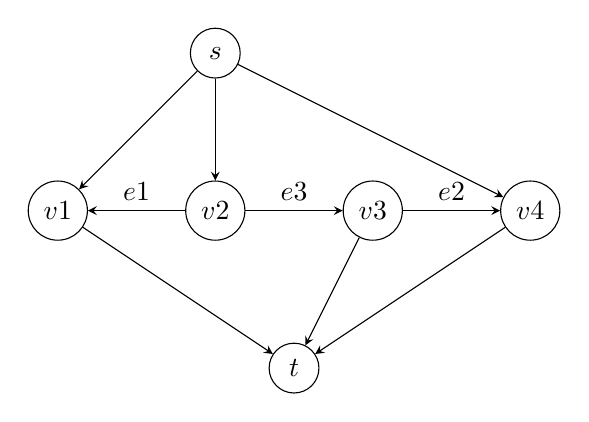
\begin{tikzpicture}[>=stealth, node distance=2cm]

        % nodes
        \node[circle, draw, minimum size=18pt] (s) at (0,2) {$s$};
        \node[circle, draw, minimum size=18pt] (v1) at (-2,0) {$v1$};
        \node[circle, draw, minimum size=18pt] (v2) at (0,0) {$v2$};
        \node[circle, draw, minimum size=18pt] (v3) at (2,0) {$v3$};
        \node[circle, draw, minimum size=18pt] (v4) at (4,0) {$v4$};
        \node[circle, draw, minimum size=18pt] (t) at (1,-2) {$t$};

        % edges from s
        \draw[->] (s) -- (v1);
        \draw[->] (s) -- (v2);
        \draw[->] (s) -- (v4);

        % edges v2 -> v1 (e1)
        \draw[->] (v2) -- node[above] {$e1$} (v1);

        % edges v3 -> v4 (e2)
        \draw[<-] (v4) -- node[above] {$e2$} (v3);

        % edges v2 -> v3 (e3)
        \draw[->] (v2) -- node[above] {$e3$} (v3);

        % edges to t
        \draw[->] (v1) -- (t);
        \draw[->] (v3) -- (t);
        \draw[->] (v4) -- (t);

        \end{tikzpicture}
        \caption{A graph that may cause infinite loop in Ford-Fulkerson algorithm}        
    \end{figure}
\end{remark}

\newpage

\section{Edmonds-Karp Algorithm}
這是史上第一個被證明是 polynomial-time 的 maximum flow algorithm。



\chapter{Computational Geometry}
\section{Nearest Point Pair}